\section{導入: グラフ上のランダムウォーク}
\subsection{グラフ}
まず基礎的な概念の定義を与える.
本講義では有限単純無向グラフを単に\emph{グラフ (graph)}と呼ぶ.
すなわち, グラフとは有限集合$V$とその二元部分集合$E\subseteq \binom{V}{2}$の組 $G = (V, E)$ である.
$V$の元を\emph{頂点(vertex)}, $E$の元を\emph{辺(edge)}と呼ぶ.
特に混乱が生じない限りは辺$\{u,v\}$を省略して$uv$と記す.
二頂点$u,v\in V$が$uv\in E$を満たすとき, $u$は$v$に隣接しているという ($v$もまた$u$に隣接している).
頂点$u\in V$に対し$\deg(u) = \abs{\cbra{v \in V \colon uv\in E}}$を\emph{次数 (degree)}と呼ぶ.
全ての頂点の次数が$d$に等しいとき, $G$は\emph{$d$-正則 ($d$-regular)}であるという.
以下で定義される行列$A \in \Real^{V\times V}$を\emph{隣接行列 (adjacency matrix)}という:
\begin{align*}
  A(u,v) = \begin{cases}
    1	& \text{if }uv\in E,\\
    0 & \text{otherwise}.
  \end{cases}
\end{align*}
考えているグラフ$G$が明らかな場合は次数や隣接行列などを$\deg(u),A$などと表す.
また, 考えているグラフ$G$が曖昧であったり特別に指定したい場合は$\deg_G(u),A_G$などと表す.

グラフ$G=(V,E)$の連結性を定義する.
二頂点$a,b\in V$に対し,
  ある頂点列$v_0=a,v_1,\dots,v_{\ell-1},v_\ell = b$
  が存在して$\cbra{v_0,v_1},\dots,\cbra{v_{\ell-1},v_\ell}$が全て$G$の辺になっているとき,
  $a\sim b$と表す.
この関係は同値関係になっており, $V$を$\sim$で割った商集合$V / \sim$の各同値類$[v]$を$G$の\emph{連結成分 (connected component)}という.
商集合$V / \sim$が単一の連結成分からなるとき, $G$は\emph{連結 (connected)}であるという.

グラフ$G=(V,E)$の二部性を定義する.
ある頂点分割$V=L\sqcup R$が存在して$E\cap \binom{L}{2}=\emptyset$かつ$E\cap \binom{R}{2}=\emptyset$が成り立つとき, $G$は\emph{二部 (bipartite)}であるといい,
頂点部分集合$L,R$を$G$の\emph{部集合 (partite set)}と呼ぶ.
直感的には, $G$が二部グラフであるというのは, ある頂点分割$V=L\sqcup R$に対して
$G$の全ての辺が$L$と$R$の間を跨いでいることを意味する.
なお, 部集合への分割$V = L\sqcup R$は必ずしも一意であるとは限らない.

\subsection{グラフ上の単純ランダムウォーク} \label{sec:SRW}
ランダムウォークは高次元エクスパンダーの定義やその解析に不可欠な概念である.
そこで本節ではまず最も基本的なグラフ上の単純ランダムウォークを定義し, その基本的な性質を紹介する.
後に単純ランダムウォークを拡張した一般的なランダムウォークを導入し, その重要なクラスである
可逆なランダムウォークについて説明する.
%
\begin{definition}{単純ランダムウォーク}{SRW}
  グラフ$G=(V,E)$を考える.
  頂点集合$V$上に値をとる確率変数の列$(X_t)_{t=0,1,\dots}$であって,
  任意の$t\ge 0$, 頂点列$(v_0,\dots,v_{t-1})\in V^t$, および$v\in V$に対して
  \[
    \Pr\sbra*{ X_t = v \condition X_0=v_0,\dots,X_{t-1} = v_{t-1} } = \Pr\sbra*{ X_t = v_t \condition X_{t-1} = v_{t-1}} = \frac{1}{\deg(v_{t-1})}
  \]
  を満たすものを$G$上の\emph{単純ランダムウォーク (simple random walk)}という.
  さらに,
  \[
    P(u,v) = \begin{cases}
      \frac{1}{\deg(u)}	& \text{if }uv\in E,\\
      0 & \text{otherwise}
    \end{cases}
  \]
  で定義される行列$P \in [0,1]^{V\times V}$を\emph{遷移確率行列 (transition matrix)}と呼ぶ.
\end{definition}
%
要するに, 初期地点$X_0$を選び, 現在いる位置から一様ランダムな隣接点を選びそこに遷移するという
確率的な操作を繰り返して得られる系列が単純ランダムウォークである.
初期地点の選び方は何でもよく,
例えば$X_0$は決定的な頂点$X_0=u$であったり一様ランダムな頂点であってもよい.
%
初期頂点$X_0$の分布が決まれば各時刻$t$における$X_t$の分布は一意に定まる.
実際, $t\ge 0$に対し$x_t \in [0,1]^{V}$を$X_t$の分布とする
  (すなわち, $x_t(u) = \Pr\sbra*{X_t = u}$).
任意の$t\ge 1$に対し
\begin{align*}
  x_t(v) &= \Pr\sbra*{X_t = v} \\
    &= \sum_{u\in V}\Pr\sbra*{ X_t = v \tand X_{t-1} = u} \\
    &= \sum_{u\in V}\Pr\sbra*{ X_t = v \condition X_{t-1} = u} \Pr\sbra*{X_{t-1} = u}  \\
    &= \sum_{u\in V} P(u,v) x_{t-1}(u)
\end{align*}
という漸化式を得る.
これは$x_{t} = x_{t-1} P$とも表せる (ここで$x_t$は行ベクトルとして扱う) ので
\begin{align}
  x_t = x_0 P^t \label{eq:x_t SRW}
\end{align}
を得る.

  グラフ$G=(V,E)$の各頂点を対角に並べた$V\times V$行列を\emph{次数行列 (degree matrix)}という.
  すなわち, 次数行列$D\in \Real^{V\times V}$は
  \begin{align*}
    D(u,v) = \begin{cases}
      \deg(u)	& \text{if }u=v,\\
      0 & \text{otherwise}.
    \end{cases}
  \end{align*}
  グラフ$G$上の単純ランダムウォークの遷移確率行列$P$は, 次数行列$D$と隣接行列$A$を用いて$P=D^{-1}A$と表せる.

\subsection{単純ランダムウォークの収束性と定常分布} \label{sec:SRW convergence}
グラフ$G$上の単純ランダムウォーク$(X_t)_{t\ge 0}$を考え, 時刻$t$における分布$x_t \in [0,1]^V$の
$t\to \infty$における収束性について述べる.

まず, 分布間の距離として全変動距離を定義する.
\begin{definition}{全変動距離}{total variation distance}
  有限集合$V$上の二つの分布$\mu,\nu \in[0,1]^V$に対し, \emph{全変動距離 (total variation distance)}を
  \[
    \dtv (\mu ,\nu ) \defeq \frac{1}{2} \sum_{u\in V}\abs{\mu(u) - \nu(u)} = \frac{1}{2} \norm{\mu - \nu}_1
  \]
  で定める.
\end{definition}
全変動距離は単に$\ell^1$ノルムを$2$で割った値だが, 次の性質を持つがゆえに統計学, 情報理論, 機械学習, 計算機科学を含む様々な分野で非常に重要な役割を果たしている.
\begin{proposition}{}{}
  有限集合$V$を考え, 分布$\pi\in[0,1]^V$と部分集合$U\subseteq V$に対し$\pi(U)\defeq\sum_{u\in U}\pi(u)$とする.
  任意の二つの分布$\mu,\nu\in[0,1]^V$と任意の部分集合$U\subseteq V$に対して
  \[
    \abs*{ \mu(U) - \nu(U) } \le \dtv(\mu,\nu).
  \]
\end{proposition}
すなわち,
全変動距離が小さいということは任意の事象の発生確率の差が小さいことを意味する.
なお, この不等式はタイトである.
実際, $U=\cbra*{ u\in V \colon \mu(u) > \nu(u) }$とすれば等号が成り立つ.

ランダムウォークの分布$x_t$がある分布$\pi\in[0,1]^V$に収束するならば, 分布の漸化式$x_t = x_{t-1}P$より収束先の分布$\pi$は
\begin{align}
  \pi = \pi P \label{eq:SRW pi equation}
\end{align}
を満たすはずである.
%
\begin{definition}{定常分布}{SRW stationary distribution}
  グラフ$G=(V,E)$に対し, \cref{eq:SRW pi equation}を満たす$V$上の分布$\pi\in[0,1]^V$を単純ランダムウォークの\emph{定常分布 (stationary distribution)}と呼ぶ.
\end{definition}
%
単純ランダムウォークの定常分布は必ず存在し, その一つは
\begin{align}
  \pi(u) = \frac{\deg(u)}{2|E|}. \label{eq:SRW stationary distribution}
\end{align}
で与えられる.
しかし定常分布は一意とは限らない.
\begin{figure}
  \begin{center}
  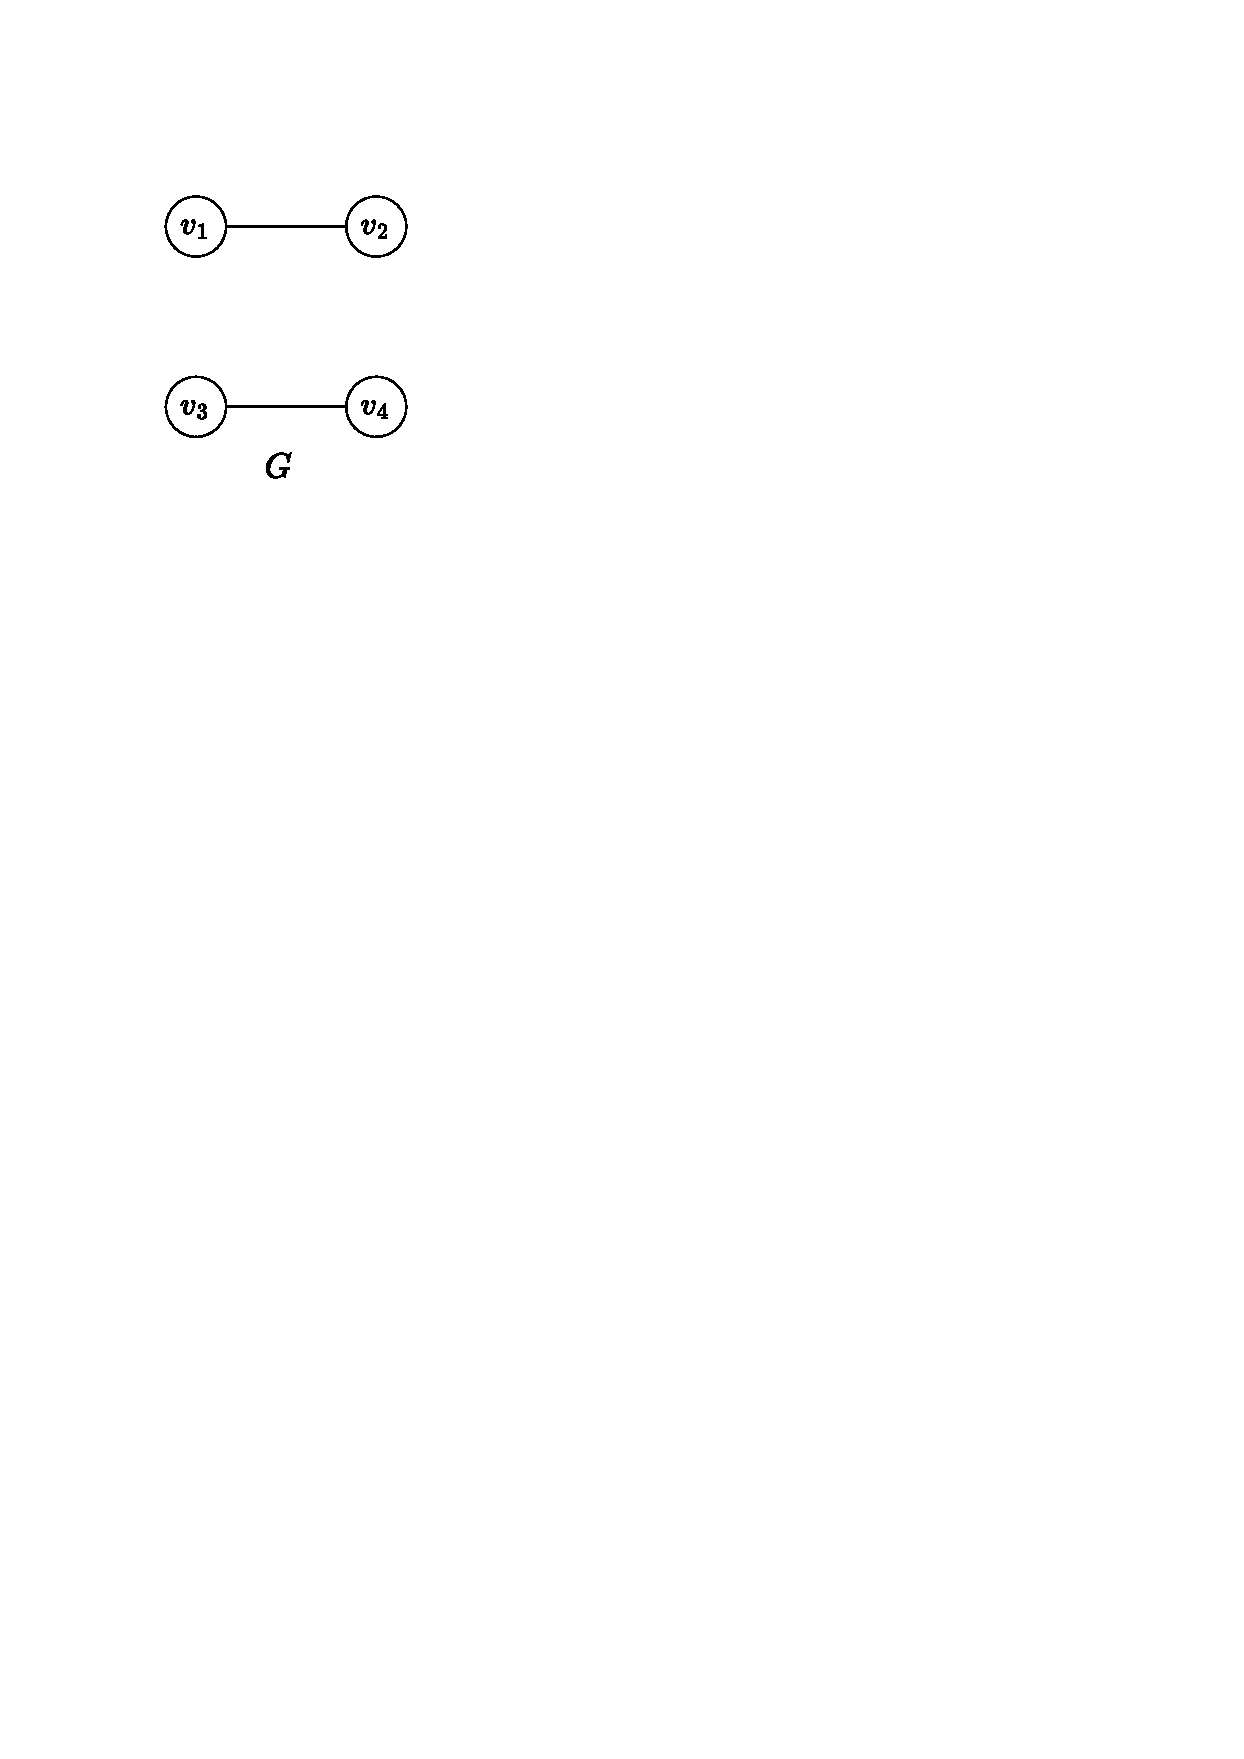
\includegraphics[width=4cm]{images/graph1.pdf}
  \caption{定常分布$\pi$が一意でない例.  \label{fig:graph1}}
  \end{center}
\end{figure}
例えば\cref{fig:graph1}に表されるグラフは定常分布として$\pi=(0,0,1/2,1/2),(1/2,1/2,0,0),(1/4,1/4,1/4,1/4)$などが考えられる.
一般に非連結なグラフを考えると$\pi = \pi P$という制約は各連結成分ごとの独立な制約に分解できてしまうので, それに対応する$\pi$の成分を$0$にしてしまうことができる.
一方でグラフ$G$が連結ならばそのような分解は存在しないので\cref{eq:SRW pi equation}を満たす$\pi$は定数倍を除いて一意に定まり, 正規化すると\cref{eq:SRW pi equation}になる.

グラフ$G$上の単純ランダムウォークの分布$x_t$の一意収束性を考える.
まず, 一意収束性が満たされないような条件を考えてみよう.
\begin{itemize}
  \item 単純ランダムウォークは同じ連結成分内でしか遷移しない. 従ってグラフ$G$が非連結ならば初期頂点$X_0$の場所によって$x_t$は異なってしまう (定常分布の非一意性).
  \item グラフ$G$が二部グラフならば, 時刻$t$の偶奇によってランダムウォークがどちらの部集合に属するかが入れ替わるので, $x_t$は収束しない.
\end{itemize}
%
実は, 収束性を阻害するのは上の二つのケースのみであることが知られている (証明は割愛).
%
\begin{theorem}{単純ランダムウォークの収束性}{SRW convergence}
  任意のグラフ$G$上の単純ランダムウォークは定常分布を一つ以上持つ.
  さらに
  \begin{itemize}
    \item グラフ$G$が連結ならば定常分布は一意であり, \cref{eq:SRW stationary distribution}で与えられる.
    \item グラフ$G$が二部グラフでないならば, 任意の初期頂点の分布$x_0$に対してある定常分布$\pi$が存在して$\dtv(x_t,\pi)\to 0$ ($t\to\infty$)を満たす.
  \end{itemize}

  特に, グラフ$G$が連結かつ非二部ならば単純ランダムウォークの分布は\cref{eq:SRW stationary distribution}で与えられる分布$\pi$に一意収束する.
\end{theorem}


\subsection{一般のランダムウォークの定義と一意収束性} \label{sec:Markov chain}
  \cref{sec:SRW}, \ref{sec:SRW convergence}ではグラフ上の単純ランダムウォークという特定の確率過程を定義し, その収束性を論じてきた.
  今後は辺集合上のランダムウォークやより一般に単体複体の面上のランダムウォークも考えていくため,
  より一般のランダムウォークを定義し, その分布の収束性や定常分布について説明する.

  一般に「ランダムウォーク」という用語は文脈によって様々である.
  例えば物理学や金融の文脈でブラウン運動を離散化したモデルを考える際は
    数直線上を等確率で左右どちらかに移動する粒子の軌跡をランダムウォークと呼ぶことがある.
  一方でネットワーク解析の文脈ではグラフ上の単純ランダムウォークをランダムウォークと呼ぶこともある.
  本講義では斉時性をもつ有限状態離散時間マルコフ連鎖をランダムウォークと呼ぶ.
  %
  \begin{definition}{ランダムウォーク}{random walk}
    有限集合$V$と確率行列\footnote{各行和が$1$となる非負行列を\emph{確率行列(stochastic matrix)}と呼ぶ.}$P\in[0,1]^{V\times V}$に対し,
    $V$上に値をとる確率変数列$(X_t)_{t\ge 0}$であって, 任意の$t\ge 0$, 頂点列$(v_0,\dots,v_{t-1})\in V^t$,
    および$v\in V$に対して
    \[
      \Pr\sbra*{X_t = v \condition X_0 = v_0,\dots,X_{t-1} = v_{t-1}} = \Pr\sbra*{X_t = v \condition X_{t-1} = u} = P(u,v)
    \]
    を満たすものを$V$上の\emph{ランダムウォーク}という.
    特に確率行列$P$をランダムウォーク$(X_t)_{t\ge 0}$の\emph{遷移確率行列}と呼ぶ.
  \end{definition}
  %
  分布$x_t$の収束性の議論は次のように展開される:
  \begin{definition}{既約性、非周期性}{}
    遷移確率行列$P \in [0,1]^{V\times V}$をもつランダムウォークを考える.
    \begin{itemize}
    \item 任意の頂点対$u,v\in V$に対しある$t \ge 0$が存在して$P^t(u,v)>0$を満たすとき, ランダムウォーク$(X_t)_{t\ge 0}$は\emph{既約 (irreducible)}であるという.
    \item 各頂点$u\in V$に対し, 有向閉路長の集合$L_u = \cbra*{ t \ge 1 \colon P^t(u,u) > 0}$を考え, その最大公約数を頂点$u$の\emph{周期 (period)} と呼ぶ. 全ての頂点の周期が$1$であるとき, ランダムウォーク$(X_t)_{t\ge 0}$は\emph{非周期的 (aperiodic)}であるという.
    \item 集合$V$上の分布$\pi\in[0,1]^V$であって$\pi = \pi P$を満たすものを\emph{定常分布 (stationary distribution)}と呼ぶ.
    \end{itemize}
  \end{definition}
%
  既約性は任意の頂点対$u,v$に対し$u$からスタートしたランダムウォークが$v$に到達可能であることを意味している.
  これは単純ランダムウォークにおけるグラフの連結性に対応している
    (一般のランダムウォークでは辺の向きも考慮しなければならない点が異なっている).

  非周期性は, 単純ランダムウォークにおける非二部性に対応する.
  二部グラフ上の単純ランダムウォークは, 無向辺に沿った長さ$2$の閉路も含めて全ての閉路長が偶数であるから全頂点の周期は偶数となる.
  一般のランダムウォークを考える場合は有向辺も考えるため, 閉路長が他の倍数になりうる.
  例えば遷移確率行列が
  \[
    P = \begin{bmatrix}
      0 & 1 & 0 \\
      0 & 0 & 1 \\
      1 & 0 & 0
    \end{bmatrix}
  \]
  で与えられるランダムウォークは全ての有向閉路の長さは$3$の倍数である.
  このような場合もやはりランダムウォークの分布$x_t$は収束しないことがわかる.
  非周期性はこのようなケースを排除するという意味を持つ.

  任意のランダムウォークは必ず定常分布をもつ.
  詳細は省くがこれは以下の議論から証明できる:
    \begin{itemize}
    \item 定常分布$\pi$は転置行列$P^{\top}$の固有値$1$の固有ベクトルに対応する.
    \item $P$と$P^\top$の固有値は全て同じ (転置をとっても行列式は変わらないから)であり, 最大固有値$1$を持つ.
    \item Perron--Frobeniusの定理から$P^\top$の最大固有値$1$に対応する固有ベクトルの成分は非負なので, 正規化すると分布になる.
    \end{itemize}
  %
  単純ランダムウォークに対する収束性の結果(\cref{thm:SRW convergence})は次のように拡張される.
  %
  \begin{theorem}{一般のランダムウォークの収束性}{random walk convergence}
      遷移確率行列$P$を持つ$V$上の任意のランダムウォークは定常分布$\pi \in [0,1]^V$を持つ.
      さらに,
      \begin{itemize}
      \item ランダムウォークが既約的ならば, 定常分布$\pi$は一意に存在する.
      \item ランダムウォークが非周期的ならば, 任意の初期分布$x_0$に対してある定常分布$\pi$が存在して$\dtv(x_t,\pi)\to 0$ ($t\to\infty$)が成り立つ.
      \end{itemize}

      特に, 既約的かつ非周期的なランダムウォークの分布はある定常分布に一意収束する.
  \end{theorem}

  本講義では以後, 単にランダムウォークと言った場合, 特に断りのない限り常に既約的かつ非周期的であると仮定する.

\subsection{混交時間}
\cref{thm:random walk convergence}ではランダムウォークの一意収束性の条件を与えた.
では, その収束の速さはどれくらいだろうか?
この問題は日常的には例えば次のような状況で現れる:
\begin{itemize}
  \item トランプカードで遊ぶとき, 何回シャッフルすればカードが「混ざり合う」か?
  \item 料理で調味料をスープに入れたとき, 何回かき回せば味が「混ざり合う」か?
\end{itemize}

ここでは「混ざり合う」とは定常分布への全変動距離の意味での収束性で定義し,
ランダムウォークの混交時間を次で定義する:
\begin{definition}{混交時間}{mixing time}
  定常分布$\pi \in [0,1]^V$を持つランダムウォーク$(X_t)_{t\ge 0}$を考え, $t\ge 0$に対し
  $x_t \in [0,1]^V$を時刻$t$における$X_t$の分布とする.
  正の実数$\varepsilon > 0$に対し, $\varepsilon$-混交時間$\tmix(\varepsilon)$を
  \[
    \tmix(\varepsilon) \defeq \inf\cbra*{ t \ge 0 \colon \dtv(x_t, \pi) \le \varepsilon}
  \]
  とする.
  また, $(1/2)$-混交時間を単に\emph{混交時間 (mixing time)}と呼ぶ.\footnote{$1/2$という数字に特に本質的な意味はない.}
\end{definition}

本講義では全体を通じてランダムウォークの混交時間(特にその上界)を評価することに取り組む.
次のロードマップに沿って講義を進める.
\begin{enumerate}
\item まず, グラフ上の単純ランダムウォークの混交時間をその固有値の性質を使って評価する.
\item 特に, 固有値の性質が「良い」グラフをエクスパンダーグラフと呼ぶ.
\item 次に単体複体上のランダムウォークを定義し, その混交時間を同様に固有値を用いて評価する.
\item エクスパンダーグラフと同様に, 固有値の性質が「良い」単体複体を高次元エクスパンダーと呼ぶ.
\item 最後にマトロイドと呼ばれる非常に重要な単体複体の固有値に関する性質を明らかにし, 重要な未解決問題であったMicali--Vazirani予想を証明する.
\end{enumerate}
